\chapter{SISTEM REFERENSI KOORDINAT}

Pada kenyataannya bumi berbentuk seperti bola (3 dimensi) dengan permukaan yang tidak beraturan (Geoid). Untuk dapat menunjukkan lokasi suatu titik, garis, dan luasan di permukaan bumi diperlukan suatu bentuk matematis yang paling dekat dengan bentuk bumi yang sebenarnya, yaitu elipsoid.

Secara umum, terdapat 2 (dua) jenis koordinat yang sering digunakan, yaitu :

\begin{itemize}
  \item \textbf{Sistem Koordinat Geografis (Lintang - Bujur) / \textit{Geographic Coordinate System}}
  
    Pada sistem koordinat ini, bumi dibagi menjadi 360 (tiga ratus enam puluh) bagian, tiap bagian bernilai 1\degree, dan titik nol derajat adalah di Greenwich, Inggris. Disamping itu, garis khatulistiwa juga merupakan garis bujur 0\degree yang membagi dua wilayah, Di atas khatulistiwa sebagai wilayah utara dan di bawah khatulistiwa sebagai wilayah selatan. Dalam aplikasinya, wilayah selatan akan diberi simbol (-) minus, sedangkan (+) untuk wilayah utara. Sistem koordinat geografis seperti terlihat pada gambar \ref{fig:koordinatgeografis}
    
    \begin{figure}[H]
      \centering
      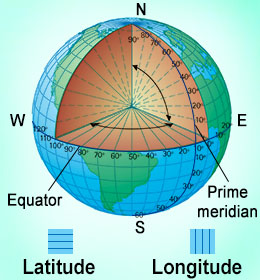
\includegraphics[scale=1]{./resources/015-koordinat-geografis}
      \caption{Koordinat Geografis}
      \label{fig:koordinatgeografis}
    \end{figure}
  
  \item \textbf{Sistem Koordinat Terproyeksi / \textit{Projected Coordinate System}}
  
    Apabila bentuk elipsoid disajikan dalam bidang datar. Maka diperlukan upaya transformasi dari bentuk 3D ke bentuk 2D melalui sistem proyeksi, seperti terlihat pada gambar \ref{fig:macamproyeksipeta}
    
    \begin{figure}[H]
      \centering
      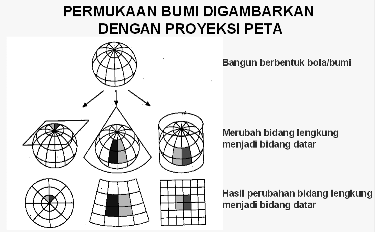
\includegraphics[scale=1]{./resources/016-macam-bidang-proyeksi-peta}
      \caption{Macam Bidang Proyeksi Peta}
      \label{fig:macamproyeksipeta}
    \end{figure}
    
    Tidak ada satu proyeksi yang bisa mempertahankan geometri asli. Semua proyeksi mempunyai distorsi geometri, namun masing-masing jenis proyeksi mempertahankan sifat aslinya, misalnya proyeksi yang mempertahankan luas permukaan (\textit{equivalen}), bentuk yang tetap (\textit{conform}), dan jarak yang tetap (\textit{ekuidistan}).
    
    Sistem proyeksi yang umum digunakan di Indonesia adalah \textbf{UTM (Universal Transverse Mercator)}. Untuk UTM, bumi kemudian dibagi ke dalam beberapa zona, antara 01 sampai dengan 60 dengan satuan meter. Pada sistem koordinat bumi akan dibagi menjadi dua bagian, di atas khatulistiwa sebagai bagian utara dengan simbol (N) serta di bagian selatan khatulistiwa di beri simbol (S).
    
    Sistem referensi koordinat yang paling cocok untuk seluruh wilayah di Indonesia adalah \textit{Geographic Coordinate System} yaitu WGS1984 (WGS84 / EPSG:4326). Sedangkan untuk wilayah satu provinsi atau lebih kecil sistem referensi koordinat yang paling cocok adalah \textbf{sistem koordinat terproyeksi} yaitu UTM WGS84. Contoh, untuk Jogja dan Jawa Tengah menggunakan UTM Zona 49S (WGS84 / UTM Zone 49S / EPSG:32749), seperti terlihat pada gambar \ref{fig:utmindonesia}.
    
    \begin{figure}[H]
      \centering
      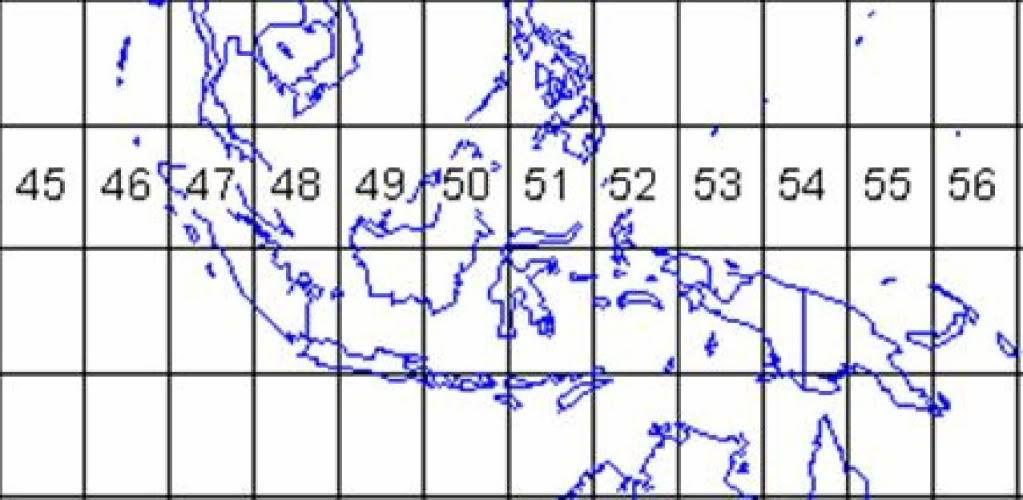
\includegraphics[width=1\textwidth]{./resources/017-utm-indonesia}
      \caption{Zona UTM di Indonesia}
      \label{fig:utmindonesia}
    \end{figure}
    
  \item \textbf{Sistem Referensi Koordinat / \textit{Coordinate Reference Systems (CRS)} di dalam QGIS}
  
    Dalam QGIS, sistem proyeksi Sistem Referensi Koordinat yang berbeda ditransformasikan secara otomatis menggunakan fitur \textit{on-the-fly} (OTF). Fitur ini memungkinkan pengguna untuk menampilkan \textit{layer} dengan CRS yang berbeda dan membuat \textit{layer-layer overlay} dengan benar. Namun terkadang kita memperoleh \textit{shapefile} yang tidak memiliki \verb{*.prj} atau \verb{*.qpr} (\textit{unprojection file}). Jika ingin menambah \textit{shapefile} itu pada \textit{map project} QGIS akan muncul dialog untuk menentukan CRS pada \textit{layer} itu sebagai CRS sementara. 
    \end{itemize}

\end{itemize}